\subsection{Embedding}
\label{sub:embedding}
As described in \autoref{subsub:graph_equivalence}, each QUBO has a corresponding graph. This graph is constructed using D-Wave hardware: superconducting qubits represent graph nodes, couplers represent graph edges. At best, the topology of the hardware should be a complete graph. This would enable a hardware realisation of any QUBO with number of variables up to the total number of qubits in a chip - $n$. This however, would require $\frac{n(n-1)}{2}$ of couplers. For a sufficiently large $n$ this becomes a prohibitively large number considering the complexity and technical limitations of chip manufacturing. Considering the actual topologies of D-Wave chips (as described in \autoref{subsub:d_wave_hardware}) and an arbitrary QUBO one would like to solve, there arises a disparity, to some extent solved by embedding. It is a process of "fitting" a graph into the hardware topology, described with a different graph. A key concept of embedding is the representation of a single logical node with many hardware nodes (qubits). This is done by strong coupling of two or more nodes, so they behave in a same way, mimicking being the same node. For analogy, one can think of two points in an electrical circuit. If they behave the same, so when the electrical potential between them is $0$, it is equivalent to a circuit where two or more points become one.

Let us recall a graph from \autoref{fig:dwave_triangle_graph}. It is a complete graph $K_3$, a triangle. Now let us go back to the Chimera topology as shown in \autoref{fig:d_wave_chimera}. It is clear that there is no single triangle in the hardware topology of chips using Chimera structure. Even in such a simple case, embedding is necessary. \autoref{fig:dwave_embedding} shows the process conceptually. 

\begin{figure}
	\centering
	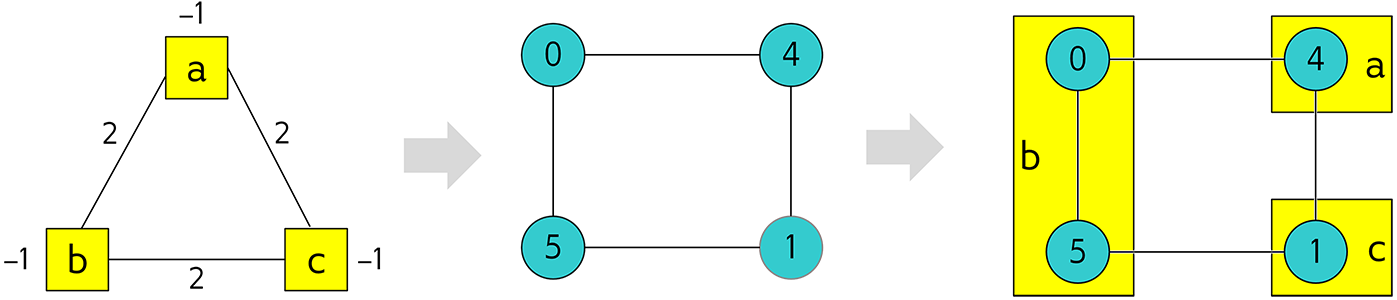
\includegraphics[width=0.8\columnwidth]{graphics/dwave_embedding.png}
	\caption{Embedding of a triangle graph into Chimera topology \cite{d-wave_inc_d-wave_2022}.}
    \label{fig:dwave_embedding}
\end{figure}

\hl{NP of embedding itself}
\hl{de-embedding}
\hl{D-Wave tools for embedding and de-embedding}